\subsection{Previous meetings}

This model can be seen as an extension to the head to head model. The model incorporates the same information at the head to head model, but for each of the previous matches. In addition to the outcome distribution and the goal distribution, this model adds the final ratings of the teams and the final result for each of the previous matches.

\begin{figure}
    \centering
    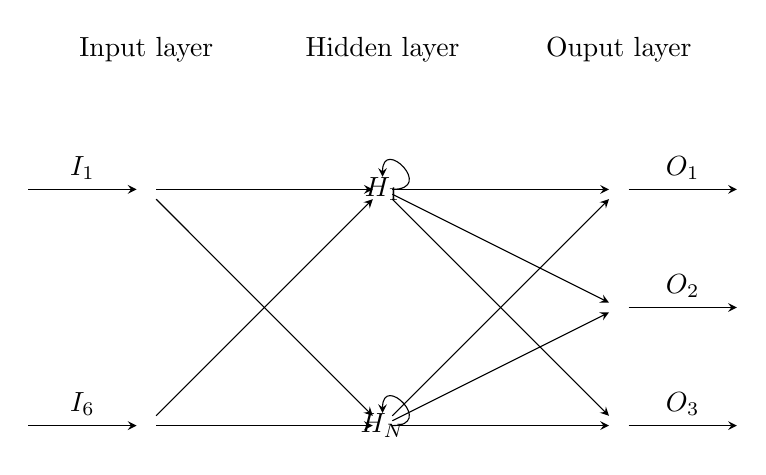
\begin{tikzpicture}[x=1.5cm, y=1.5cm, >=stealth]
        %%%%%%%%%%%%%%%%%%%%%%%%%%%%%%%%%%%%%%%%%%%%
        % Input nodes
        %%%%%%%%%%%%%%%%%%%%%%%%%%%%%%%%%%%%%%%%%%%%
        
        % Drawing
        \foreach \m/\l [count=\y] in {1,missing,2}
            \node [every neuron/.try, neuron \m/.try] (input-\m) at (0,2-\y) {};

        % Labeling
        \foreach \l [count=\i] in {1,6}
            \draw [<-] (input-\i) -- ++(-1,0)
                node [above, midway] {$I_{\l}$};
        
        
        %%%%%%%%%%%%%%%%%%%%%%%%%%%%%%%%%%%%%%%%%%%%
        % Hidden nodes
        %%%%%%%%%%%%%%%%%%%%%%%%%%%%%%%%%%%%%%%%%%%%
        
        % Drawing
        \foreach \m [count=\y] in {1,missing,2}
            \node [every neuron/.try, neuron \m/.try ] (hidden-\m) at (2,2-\y) {};
        
        % Labeling
        \foreach \l [count=\i] in {1,N}
            \node at (hidden-\i) {$H_{\l}$};
        
        \draw[->,shorten >=1pt] (hidden-1) to [out=0,in=90,loop] (hidden-1);
        \draw[->,shorten >=1pt] (hidden-2) to [out=0,in=90,loop] (hidden-2);
        
        %%%%%%%%%%%%%%%%%%%%%%%%%%%%%%%%%%%%%%%%%%%%
        % Output nodes
        %%%%%%%%%%%%%%%%%%%%%%%%%%%%%%%%%%%%%%%%%%%%
        
        % Drawing
        \foreach \m [count=\y] in {1,...,3}
            \node [every neuron/.try, neuron \m/.try ] (output-\m) at (4,2-\y) {};
        
        % Labeling
        \foreach \l [count=\i] in {1,...,3}
            \draw [->] (output-\i) -- ++(1,0)
                node [above, midway] {$O_{\l}$};
        
        
        %%%%%%%%%%%%%%%%%%%%%%%%%%%%%%%%%%%%%%%%%%%%
        % Connecting
        %%%%%%%%%%%%%%%%%%%%%%%%%%%%%%%%%%%%%%%%%%%%
        
        % Input nodes to hidden nodes
        \foreach \i in {1,...,2}
            \foreach \j in {1,...,2}
                \draw [->] (input-\i) -- (hidden-\j);
        
        % Hidden nodes to output nodes
        \foreach \i in {1,...,2}
            \foreach \j in {1,...,3}
                \draw [->] (hidden-\i) -- (output-\j);
        
        
        %%%%%%%%%%%%%%%%%%%%%%%%%%%%%%%%%%%%%%%%%%%%
        % Labeling layers
        %%%%%%%%%%%%%%%%%%%%%%%%%%%%%%%%%%%%%%%%%%%%
        \foreach \l [count=\x from 0] in {Input, Hidden, Ouput}
            \node [align=center, above] at (\x*2,2) {\l\ layer};
    \end{tikzpicture}
    \caption{Previous meetings network structure. N is the number of nodes in the hidden layer.}
    \label{fig:network-previous-meetings-to-result}
\end{figure}

\subsubsection{Input}

The following values are added for each of the previous matches:
\begin{itemize}[noitemsep]
    \item Days since the match, $exp(-\text{days since match} / 730)$. This is added in order to increase the impact of more recent matches.
    \item Goal distribution for the match.
    \item Home team final rating.
    \item Away team final rating.
    \item Final result of the match. $0$ for home victory, $0.5$ for draw, $1$ for away team victory.
\end{itemize}

For each previous match, there are six values. With up to six previous matches, there is a total of $6 * 6 = 36$ features for each match. If two teams have less than six previous matches, a list of six zeros are supplied for each missing match.

For the match between Arsenal and Manchester United May 7, 2017, the input values would be as follows:
\begin{lstlisting}[language=Python]
    [[0.451, 3/3, 0/3, 0.77, 0.63, 0.0]
    [0.293, 1/3, 2/3, 0.65, 0.71, 1.0]
    [0.199, 1/2, 1/2, 0.73, 0.71, 0.5]
    [0.133, 1/2, 1/2, 0.67, 0.67, 0.5]
    [0.071, 1/3, 2/3, 0.67, 0.71, 1.0]
    [0.049, 1/1, 0/1, 0.71, 0.64, 0.0]]
\end{lstlisting}

The hidden layer is a fully connected simple recurrent layer. \cref{fig:network-previous-meetings-to-result} shows the structure of the network. When feeding a match through the network, the previous matches are fed through the hidden layer one by one. The hidden layer output from one match is added to the input for the next.